\documentclass[9pt,twocolumn,twoside,lineno]{gsag3jnl}

\articletype{inv} % article type
% {inv} Investigations
% {msr} Mutant Screen Reports
% {gs} Genomic Selection
% {goi} Genetics of Immunity 
% {gos} Genetics of Sex 
% {mp} Multiparental Populations
\usepackage{verbatim}
\usepackage{multirow}
%\usepackage{listings}
\usepackage[cache=false]{minted}
\newcommand{\code}{\texttt}


\title{Speeding up eQTL scans in the BXD population using GPU}

\author[$\ast$]{Xiaoqi Hu}
\author[$\ast$]{Hyeonju Kim}
\author[$\ast$]{Gregory Farage}
\author[$\dagger$]{Pjotr Prins}
\author[$\dagger$]{Robert W. Williams}
\author[$\S$]{Karl W. Broman}
\author[$\ast$,1]{\'Saunak Sen}

\affil[$\ast$]{Department of Preventive Medicine, University of Tennessee Health Science Center, Memphis, TN} 
\affil[$\dagger$]{Department of Genetics, Genomics and Informatics, University of Tennessee Health Science Center, Memphis, TN} 
\affil[$\S$]{Department of Biostatistics, University of Wisconsin-Madison, Madison, WI}


\keywords{Linear Model \\ Genome Scan \\ GPU}


\runningtitle{Speeding up eQTL scans in the BXD population using GPU} % For use in the footer 

%% For the footnote.
%% Give the last name of the first author if only one author;
% \runningauthor{FirstAuthorLastname}
%% last names of both authors if there are two authors;
% \runningauthor{FirstAuthorLastname and SecondAuthorLastname}
%% last name of the first author followed by et al, if more than two authors.
\runningauthor{Hu \textit{et al.}}

\begin{abstract}
The BXD strains of mice are an important reference population for
systems biology and genetics that have been full sequenced and deeply phenotyped.
To facilitate interactive use of genotype-phenotype relationships
in this family, we sought to develop new algorithms and code to enable
high performance whole genome QTL scan for massive omics data sets of up to 1 million 
traits. By using easily parallelizable operations including
matrix multiplication, vectorized operations, and elementwise
operations, we have been able to decrease runtimes approaching real-time
computation, making this code ideal for interactive web services, such as
GeneNetwork.org. We used parallelization of different CPU threads
as well as GPUs. We found that the speed advantage of GPUs is
dependent on problem size and shape (n of cases, n of genotypes, n of traits).  
Our results provide a clear path for speeding up eQTL scans using LMMs. 
Our implementation is in the Julia programming language.
\end{abstract}

\begin{document}

\maketitle
\thispagestyle{firststyle}
\logomark
\articletypemark
\marginmark
\firstpagefootnote

% Use the \equalcontrib command to mark authors with equal
% contributions, using the relevant superscript numbers
%\equalcontrib{1}
%\equalcontrib{2}

\correspondingauthoraffiliation{1}{Corresponding author: Saunak Sen, Department of Preventive Medicine, University of Tennessee Health Science Center, Memphis, TN. sen@uthsc.edu}
\vspace{-34pt}% Only used for adjusting extra space in the left column of the first page

\noindent The BXD mouse strains are an important set of recombinant
inbred lines with deep phenotypic characterization.  Since the strains
have been genotyped and sequenced, once a set of strains is
phenotyped, the data can be immediately used for QTL (quantitative
trait locus) mapping, and associational analysis with
previously-collected phenotypes.  For ``omic'' phenotypes collected
using high-throughput technologies, additional analyses (such as
transcriptional network construction or causal mediation analyses) are
possible.  The GeneNetwork project ({\tt http://gn2.genenetwork.org})
seeks to facilitate this process by providing a searchable database of
phenotypes and genotypes in a variety of organisms (including mouse,
rat, and Arabidopsis).  It provides a suite of interactive tools for
browsing the data, QTL mapping, correlational analyses, network
construction, and genome browsing.  Our goal is to develop a real-time
backend for GeneNetwork to perform eQTL analysis (where we perform
single-trait QTL mapping for thousands of ``omic'' traits) for
important genetic reference populations such as the BXD population.

%% Computational demands in omics are growing exponentially. For
%% instance, eQTL analysis requires processing genomewide expression and
%% marker data; this can take minutes, hours or days depending on problem
%% size.  Scientists want to intereact with the results and real-time
%% processing would be valuable.  Our goal is to build a backend for
%% GeneNetwork that will enable real-time genome scans for important
%% genetic reference populations such as the BXD population.

To perform eQTL scans in the BXD population, one has to simply perform
as many genome scans as there are phenotypes.  This can be done in an
 ``embarassingly parallel'' fashion by using standard algorithms for
 QTL analysis such as those employed by R/qtl (cite).  In practice,
this is too slow, and substantial speedups are possible.  [Mention
  ideas that have been used before] For example, by using the
Haley-Knott algorithms using genotype probabilities on batches of
phenotypes with the same missing data pattern, instead of using the EM
algorithm on each phenotype individually, substantial speedups are
possible.  This is a well-known trick and is used by R/qtl.
Additionally, if only additive effects are tested, or if the
population has only two genotype categories (as in a backcross or
recombinant inbred line), then matrix multiplication can be used to
perform Haley-Knott regression \citep{shabalin2012matrix}.  

The matrix multiplication with large matrices is the most computationally intensive and time-consuming 
to perform eQTL analysis.  By dividing large matrices into small block matrices, 
one can achieve striking efficiency in matrix multiplication in conjunction with built-in BLAS in R, 
Intel Kernel Math Library (KML) in Revolution R/Matlab, or even GPU CUDA in Matlab.  
For instance, GOTO BLAS, only available in 64 bit R only, and KML allow the use of multiple CPU cores and provide 14-17 times 
better performance than built-in BLAS in R.  GPU-based computation shows 10 times better performance than 
the best algorithm for the CPU for single precision even if Matlab provides GPU CUDA but limited support to it (cite : Matrix eQTL).

%% Compare matrix eQTL GridLMM \citep{runcie2018fast}, Bolt-LMM
%% \citep{loh2015efficient}

We sought to build upon these efforts aiming to perform real-time eQTL
scans for the BXD populations.  We used the above-mentioned ideas and
examined the use of graphical processing units (GPUs) to speed these
further.  Since programming for GPUs is often non-trivial needing the
use of low-level languages such as C++, we used the Julia programming
language which offers a GPU programming capabilities while retaining
the simplicity of a high-level language such as R or Matlab.  Finally,
since most phenotype-marker associations are null, we examined the
impact of storage precision, and only returning the highest
association (LOD) score for each phenotype instead of a matrix of LOD
scores for every pair of marker and phenotypes.  With these efforts,
we find that it is possible to perform perform real-time eQTL scans
for the BXD population.

\section{Methods and Data}
\label{sec:methods:Data}

%Manuscripts submitted to G3 should contain a clear description of the experimental design in sufficient detail so that the experimental analysis could be repeated by another scientist. If the level of detail necessary to explain the protocol goes beyond two paragraphs, give a short description in the main body of the paper and prepare a detailed description for supporting information.  For example, details would include indicating how many individuals were used, and if applicable how individuals or groups were combined for analysis. If working with mutants indicate how many independent mutants were isolated. If working with populations indicate how samples were collected and whether they were random with respect to the target population.

% This data subsection is repeated in the last subsection (information and availability of Data sets)
%\subsection{BXD genotypes and phenotypes}

%Describe genotype and phenotype data here.


\subsection{Linear Model} 
 Let $y_i$ denote a vector of gene expressions for $n$
individuals in the $i$-th omics trait ( $i=1,\ldots,m$).  We
define a univariate linear model as follows:

\begin{eqnarray*}
	y_i &=& X_j \beta_j+ \epsilon_i,
	\quad \epsilon_i \sim N(0,\sigma_i^2I),
\end{eqnarray*}
where ${X}_j$ is a matrix that may include the $y-$intercept with
or without covariate(s), and the $j$-th candidate genetic marker
($j=1,\ldots,p$).  ${\beta}_j$ is a vector of the $j$-th eQTL
effects, and ${\epsilon}_i$ is random error distributed as $N(0,\sigma_i^2I)$.  Suppose $RSS_{0i}$
is a residual sum of squares under the null hypothesis of no eQTL, and $RSS_{1ij}$ is the residual sum of squares under the
alternative of existing eQTL at the $i$-th trait and $j$-th marker.  Then the LOD
score for the corresponding pair can be written as:

\begin{eqnarray*}
	LOD_{ij} &=& \frac{n}{2} \log_{10} \left( \frac{RSS_{0i}}{RSS_{1ij}} \right)\\
	&=& \frac{n}{2} \log_{10} \left( 1{-}r_{ij}^2 \right),
\end{eqnarray*}
where $r_{ij}$ is the correlation between the $i$-th trait and
$j$-th marker. Note that this only works for one-df tests.  If $Y^{\ast}$ and $G^{\ast}$ are respectively standardized 
trait ($Y$) and genotype ($G$) matrices, then the
correlation matrix is simply $$R=Y ^{\ast '}G^{\ast}.$$
%Indicate which statistical analysis has been performed and describe the method and model applied. If many genes were examined simultaneously, or many phenotypes, a multiple comparison correction should be used to control the type I error rate, or a rationale for not applying a correction must be provided. The type of correction applied should be clearly stated. It should also be clear whether the p-values reported are raw, or after correction. Corrected p-values are often appropriate, but raw p-values should be available in the supporting materials so that others may perform their own corrections. 
Figure \ref{MatrixMult} shows the data layout.
      \begin{figure}[!htb]
	
	\caption{Schematic of data and correlation calculation: $Y$ is
		the expression phenotype matrix, $G$ is the matrix of
		genotytpes, and $R=Y^{\prime}G$ is the matrix of
		correlations.  The LOD scores are a function of the
		correlation matrix.}
	\label{MatrixMult}
	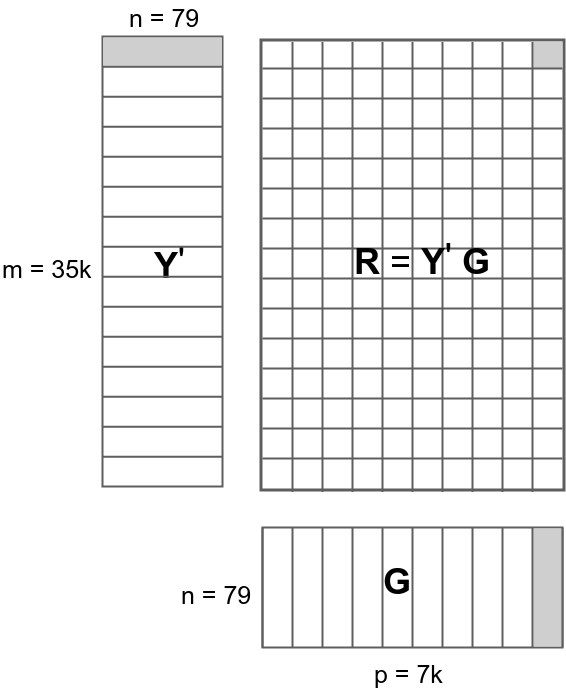
\includegraphics[scale = .4]{figs/YGmatrix.png}
\end{figure}    

\subsection{Acceleration Techniques}
We used various techniques to accelerate eQTL scan. 
\subsubsection{Multithreaded CPU operations}
% Used for multi-threaded loops whenever possible, eg. for element-wise operations. 
 Our goal is to build a backend for GeneNetwork that allows researcher to interact with data in real time. 
 Such requirement sets up the standard that the genome scan must finish within seconds.
 To bring out the best performance of CPU, we use multithreaded operations whenever possible. 
 Julia \citep{bezanson2017julia}, our choice of programming language, provide simple yet safe syntax for multithreading. 
 It is simply done by adding \code{Threads.@thread} macro to indicate to Julia that the following \code{for} loop is multhreaded region. 
 Using \code{Threads.nthreads()} function can show the number of threads in julia, and the default number of threads we use is 16 threads. 
  
 
\subsubsection{Matrix and Vectorized Operations}

% OpenBLAS for multi-threaded matrix operations. 
Since our algorithm largely depends on matrix operations, it is natural to find the fastest way to achieve best result, regardless of computing platform. 
There are various matrix libraries available for CPU, such as gslBLAS and OpenBLAS \citep{wang2013augem}. 
They target different hardware or use various techniques to get highly optimal results. 
The matrix multiplication in OpenBLAS is default multithreaded and therefore does not require extra coding effort to make the CPU version of matrix multiplication run in parallel.
We chose OpenBLAS as CPU computing library.  

Matrix multiplication and element-wise operation are algorithmically free of data and function dependency, so that they are amendable to GPU's parallel computing power.
Julia provides various packages for GPU including CUDA \citep{Nickolls:2008:SPP:1365490.1365500}, OpenCL bindings. 
Our chosen hardware for GPU is from Nvidia, which requires its proprietary library CUDA. 
Besides the hardware requirement, CUDA is also mature and has been recognized in the scientific computing community. 
\textit{cuBLAS} \citep{cublas} library is a fast GPU implementation of the BLAS from Nvidia. 
For matrix operations on GPU, we used cuBLAS library. 

Not only do we want to see how much speed up we can get from using GPU, but we also experiment whether the shape of matrix will affect the speedup. 
Of course, most of the time, one can not pick the size and shape of data in a matrix form, 
but such information would help researchers as a rough guidance of whether it is worth considering the GPU option before investing programming effort for GPU. 
We run matrix multiplication with different shapes of matrices, and compared the running time of CPU and GPU. 
CPU time is measured in matrix multiplication from OpenBLAS library using 16 threads. 
GPU time includes all overhead of using GPU, which involves device launch, data transfer and all necessary API calls.
In order to make a fair comparison between CPU and GPU, we need to use maximum strength of both and include all necessary cost. 

The experiment setup is to multiply two input matrices, A(m$\times$n), and B(n$\times$p), and produce an output matrix C(m$\times$p).  
The range of m, n and p is between 2\textsuperscript{4} and 2\textsuperscript{17} in log scale.
Due to the GPU hardware limitations, we can only compare the result when the size of input and output (I/O size) matrix, in total, is less than 16 GB. 
The result is shown in Figure \ref{GPUCPUShape}. 
The X axis of Figure \ref{GPUCPUShape} is the dimensions of matrix whose I/O size is over 12 GB.
This is because using GPU involves a lot of overhead. 
Such overhead can only be justified by processing large data sets. 
The Y axis is the speedup of GPU compared to CPU in log scale.  
From this figure, the matrices whose shapes are closer to square matrices get better speedups from GPU.
Matrix multiplication is up to 5 times faster on GPU compared to that on 16 threaded CPU. 


\begin{figure}[!htb]
	\centering
	\caption{Variation of GPU vs CPU speedup with matrix shape
	}
	\label{GPUCPUShape}
	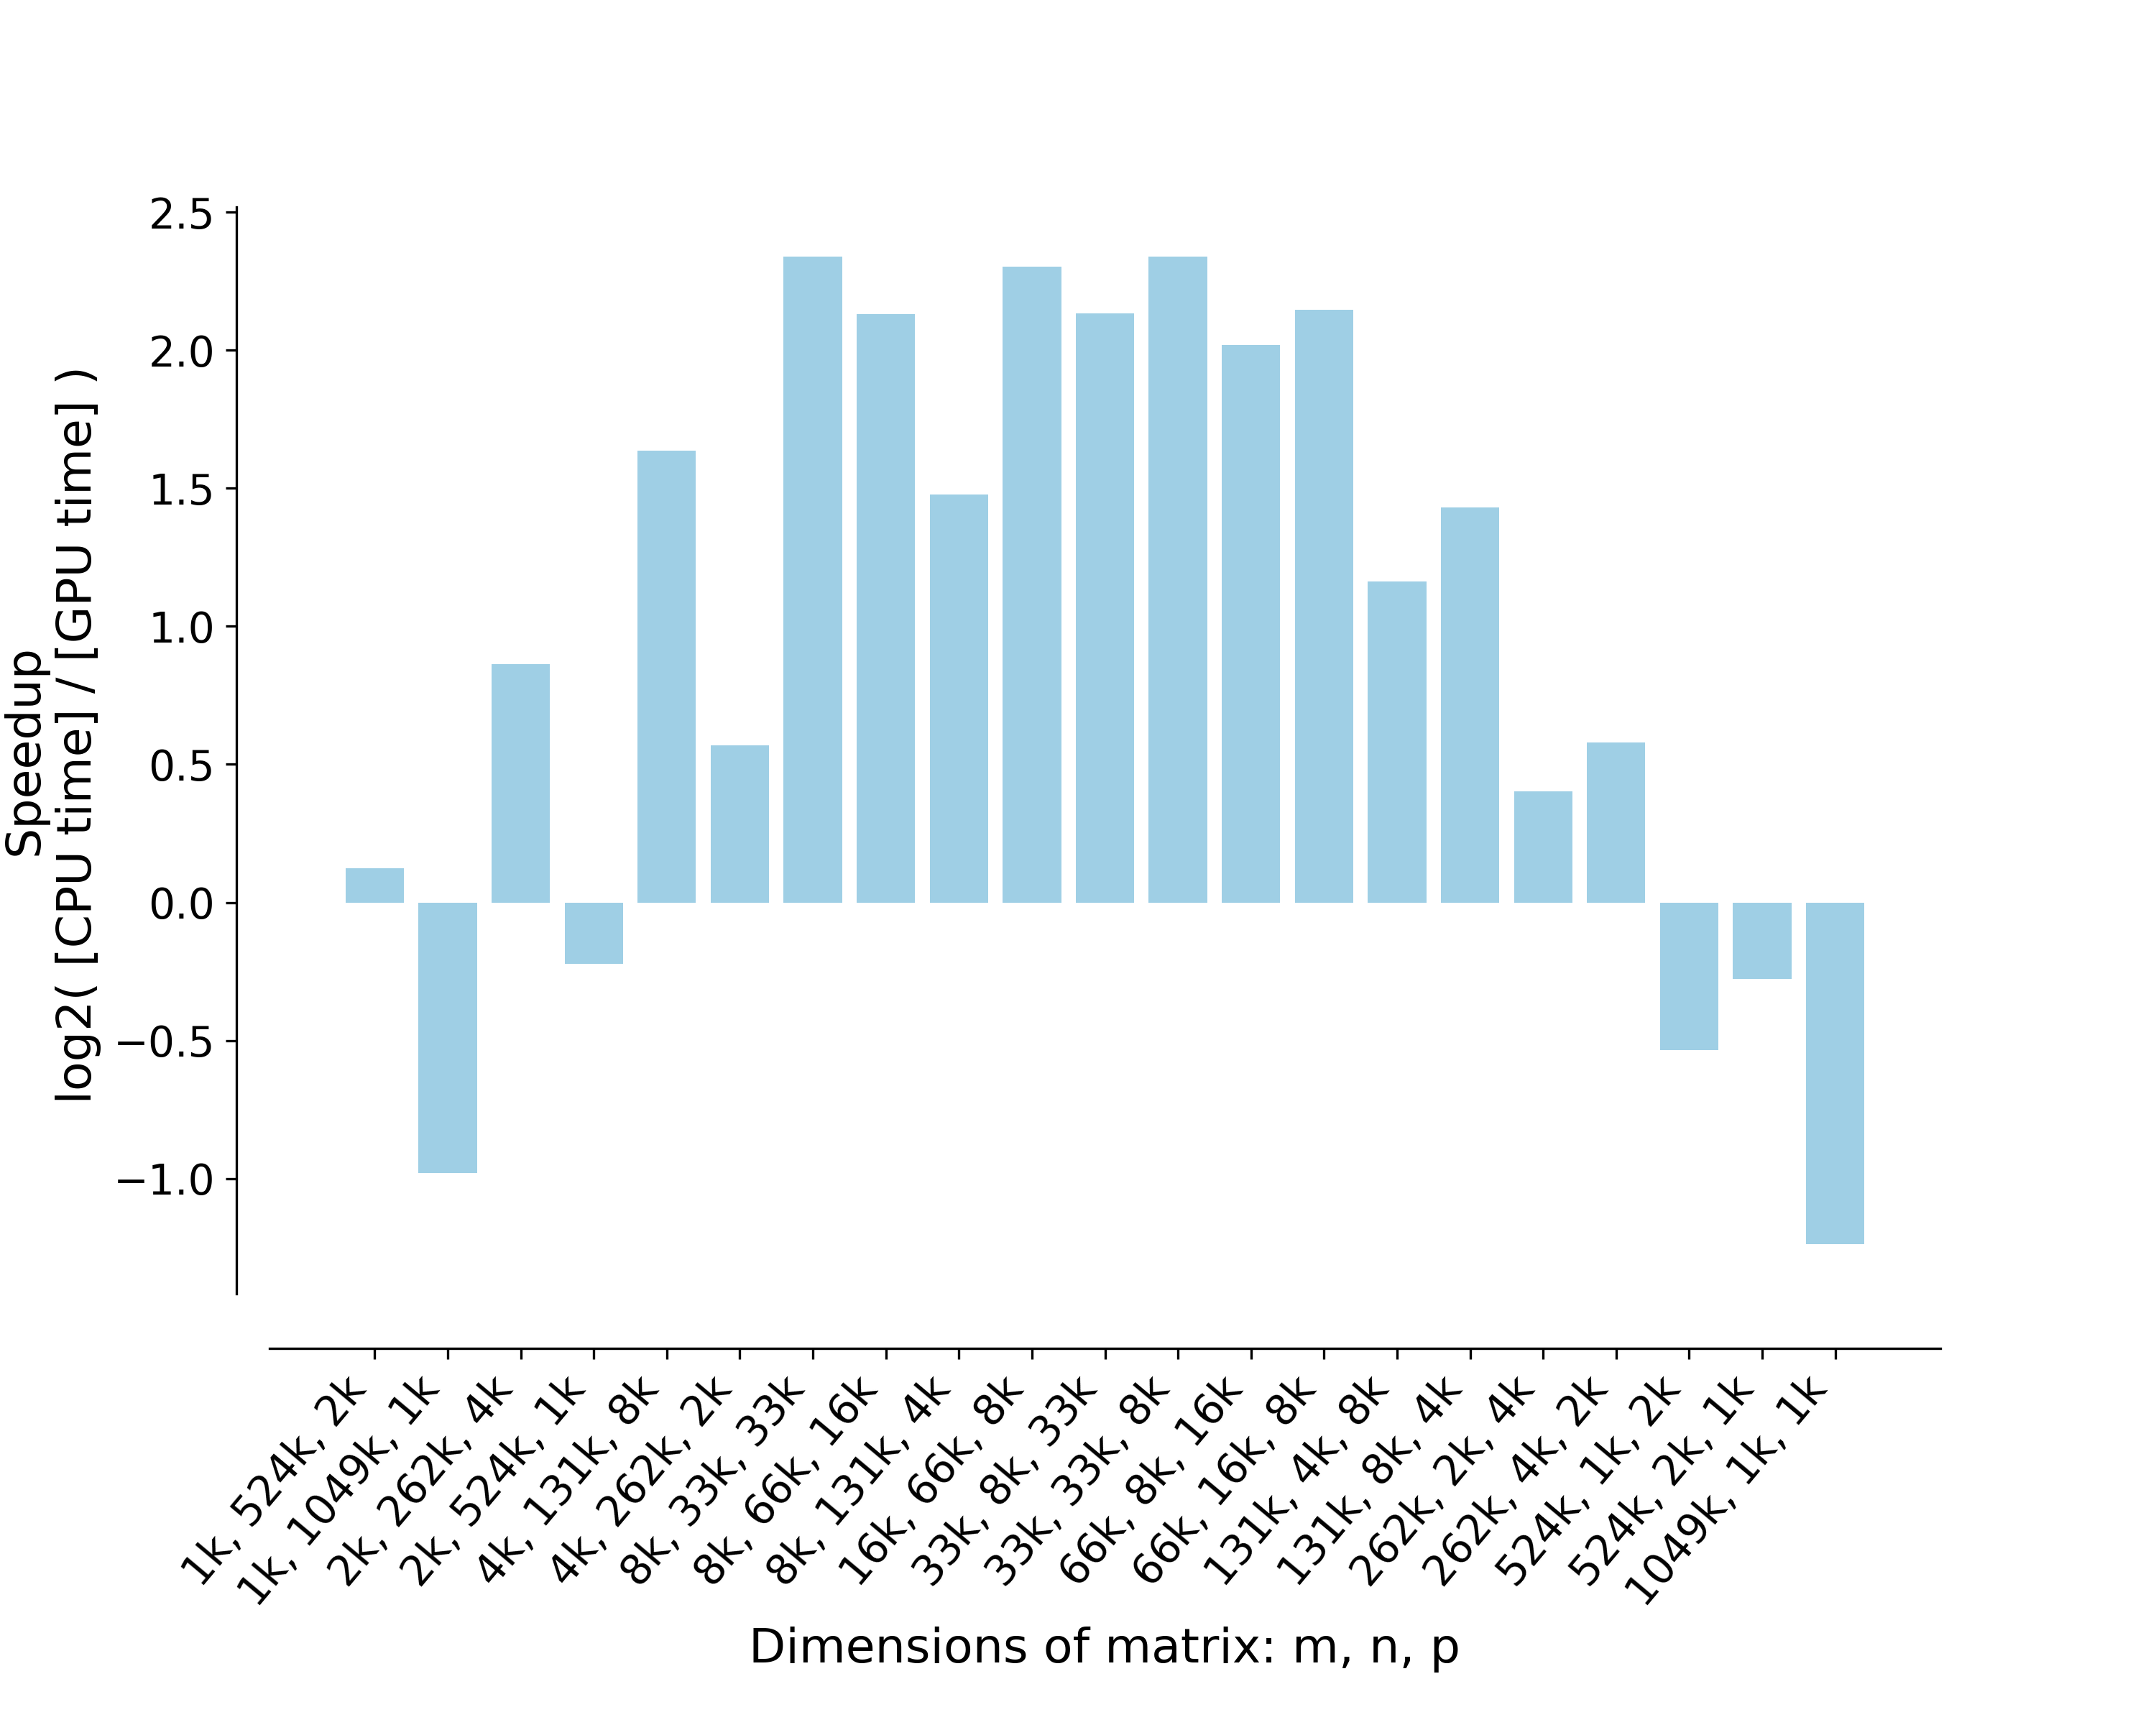
\includegraphics[scale = 0.35]{figs/speedup.png}
\end{figure} 

 
\subsubsection{Single precision}
% Faster and memory efficient; may be less accurate, but acceptable for quick scan
Precision means the smallest difference between two representable numbers.
Floating point numbers, in scientific computing, are usually stored in double precision. 
Double precision takes up 8 bytes in memory, while single precision takes up 4 bytes. 
In addition to the difference in storing size, the speed for calculation using single and double precisions also varies 
depending on the hardware.  For example, the GPU throughput (number of floating point calculation per second, measured in FLOPS)
for double precision is 1/32 of single precision on a Nvidia GTX 1050 GPU, and 1/4 on a Nvidia Tesla K80. 
Differences in optimization techniques, underlying architecture cause such performance gap. 
Considering the storage size, data transfer speed and throughput, single precision brings multiple benefits when precision is not the priority concern. 


\subsubsection{GPU operations}

%Specialized computations such as matrix multiplications and element-wise operations; requires additional programming effort
Originally used in graphics, GPU has taken off as a general computing device in recent years because of its massive number of cores at a lower price range, and fast GPGPU libraries such as CUDA and OpenCL.
Based on our profiling result, the time consuming parts of our genome scan method are matrix multiplication and element-wise operations. 
Both are amendable to GPU's heterogeneous computing architecture, since they have no data race conditions and low data dependencies. 
However, GPU also has its own limitations. 
To truly utilize the maximum computing power of GPU, one needs to think creatively to work around such limitations from GPU. 
For example, during our experiment, memory transfer between host and device is really slow. 
Profiling result shows that 98\% of total genome scan time is spent on memory transfer. 
To cope with this limitation, instead of off-loading the entire correlation matrix, we use GPU to calculate the max LOD score of each phenotype and output the max. 

\subsubsection{Julia language}
%Programming simplicity of interpreted languages with speed approaching compiled languages; GPU programming and linear algebra straightforward
In our experiment of matrix multiplication, Julia's speed is comparable to C/C++. 
However, the low learning curve, clean syntax, as well as support to GPU programming libraries such as CUDAnative \citep{CUDAnative.jl-2018} and CuArrays affords much lower programming efforts compared to C/C++.
Compared to writing GPU functions in C/C++, writing in Julia is cleaner and easier because it requires much less boiler plate code.
Below is some code snippets to demonstrate GPU code, calling library or writing custom kernel in Julia. 

\inputminted{julia}{code/gpu.jl}
%TODO: Add reference to CUDAnative and CuArrays

\subsection{Information and Availability of Datasets}

We downloaded BXD Genotype Database (GN Accession: GN600) and two sets of gene expression data, 
UTHSC Affy MoGene 1.0 ST Spleen (GN Accession : GN283)
and  UMUTAffy Hippocampus Exon (GN Accession: GN206) from GeneNetwork to test our method.  
The genotype file includes 7321 markers by 198 BXD strains, the spleen consists of 79 BXD strains by 35556 transcripts, 
and the hippocampus does 70 BXD strains by 1,236,087 probes/probe sets.  
Genotypes were subsetted by strains, pseudo markers were generated and added only to hippocampus data, 
and genotype probabilities were computed accordingly.  We thus used genotypes of 79 strains by 7321 markers for the spleen data, and 
those of 70 by 8570 for the hippocampus data for eQTL scan.  The whole cleaning process was performed using R/qtl, R/qtl2.



\begin{table*}[htbp]
	\renewcommand{\familydefault}{\sfdefault}\normalfont
	\centering
	\caption{\bf Time comparison between CPU and GPU}
	\begin{tableminipage}{\textwidth}
		\begin{tabularx}{\textwidth}{XXXXX}
			\hline
			\header Dataset & Method & Precision & CPU only   & CPU \& GPU  \\
			\hline
			\multirow{4}{*}{Spleen Data}                                                & \multirow{2}{*}{No Find Max} & Single    & 0.36s  & 0.41s \\
			&                              & Double    & 0.55s  & 0.80s \\
			& \multirow{2}{*}{Find Max}    & Single    & 0.46s  & 0.06s \\
			&                              & Double    & 0.71s  & 0.08s \\
			\hline
			\multirow{2}{*}{\begin{tabular}[c]{@{}c@{}}Hippocampus\\ Data\end{tabular}} & \multirow{2}{*}{Find Max}    & Single    & 17.64s & 2.26s \\
			&                              & Double    & 26.77s & 3.51s \\
			\hline
			
		\end{tabularx}
		\footnotetext[1]{There are overhead of using GPU, such as data transfer and setting up context, the timing shown for CPU \& GPU here included all overhead for fairness. We ran the genome scan process 10 times and choose the median to remove randomness of each run, and the warm up time of GPU.}
		\label{tab:speedup-table}
	\end{tableminipage}
\end{table*}

 
\section{Results} 

\subsection{Benefit of using linear model}
Our method uses the linear model and simplified the genome scan process to basic matrix operations. 
The timing of our method is shown in Table \ref{tab:speedup-table}. 
The execution time without finding the maximum LOD score of phenotype using double precision is 0.55 second if we only use CPU. 
Getting the same result using the same dataset from R/qtl took about 36.5 seconds. 

\subsection{Benefit of using single precision}
Table \ref{tab:speedup-table} also shows the execution time using single and double precisions. 
In all cases, genome scan using single precision runs faster than double precision. 
Using single precision provides benefits in 3 aspects: memory storage, data transfer, and arithmetic calculation. 

\subsection{Benefit of using GPU}
In parallel computing, Amdahl's law is used to find the theoretical maximum speedup by improving a particular part of a program.  
For example, if a program takes ten minutes for a serial processor, and a function that takes nine our of those ten minutes can be parallelized, and then, the theoretical speedup, no matter how many processors are used, can not be more than ten times because the minimum execution time of this program is one minute. 
Therefore, profiling the entire genome scan process is prerequisite to the optimization. 
Often, profiling would consider space and time complexity. 
Our primary concern is the time taken by each function, and therefore only timing information is considered in our profiling. 
We used Julia's built-in Sampling Profiler to find our target function for GPU because it is less intrusive compared to the other profiling methods. 

The genome scan process includes the following steps:
\begin{itemize}
	\item Calculate standardized matrices ($G^{\ast}$, $Y^{\ast}$) for input matrices ($G$, $Y$)
	\item Get a correlation matrix ($R$) by multiplying the standardized matrices
	\item Calculate LOD scores 
\end{itemize}
Our profiling result shows that both of the second and third steps take up 90\% of the time and involve parallelizable matrix operations.  Hence, they are our candidates for GPU acceleration.
To make a fair comparison for CPU and GPU, the timing shown in Table \ref{tab:speedup-table} is the total execution time for genome scan. 
The \textit{No Find Max LOD} method shows the timing when running the scan with \textit{CPU only} and \textit{CPU\&GPU}.
As the table shows, the CPU\&GPU combination did not show any improvement over the serial version (CPU only) in terms of the performance time.  That is, the former is rather slower than the latter regardless of precision for the data type.
We used a GPU profiler \textit{nvprof} \cite{nvprof}
to investigate what is the bottleneck of GPU. 
The result is, 98\% of the time is spent on data transfer from GPU to CPU (device to host).
As shown in Figure \ref{MatrixMult}, the input matrices Y' and G are small compared to the output matrix R.
For BXD spleen dataset, the Y' and G matrix is about 40MB %TODO: double check on this number 
while R matrix is about 4GB. 
Data offloading is the main bottleneck for our GPU implementation. 

To cope with this limitation of GPU, we further developed \textit{Find Max LOD} method because the main interest of genome scan is to find the maximum LOD score of every trait. 
This step is highly parallelizable, can utilize GPU's massive cores, and, at the same time, reduces the amount of data that needs to be transferred back to host. 
Table \ref{tab:speedup-table} shows that \textit{Find Max LOD} method for spleen data reduces CPU\&GPU execution time down to 0.079 second when using double precision. 
Compared to CPU only, which took 0.55 seconds, this GPU modification provides 7 times speedup. 
As we mentioned earlier, since we are porting the computation to GPU which took 90\% of the total execution time, according to Amdahl's Law, the theoretical maximum speed up is 10 times. 
We got 7 times speed up for genome scan using GPU. 
For hippocampus data, which contains over 1 million phenotypes, the GPU Find Max implementation took 3.51 seconds for double precision, and 2.26 seconds for single precision. 
As a backend service to a website, this wait time is much more preferable than the CPU timing for real time interactions. 

\subsection{Software Availability}
The source code for this package is publicly available on Bitbucket: \url{https://bitbucket.org/Xiaoqi-hu/lm-gpu}.
This repository contains three folders: \textit{data}, \textit{src} and \textit{test}. 
Using Julia language and running \code{test.jl} in \textit{test} folder will run our method using either spleen data or hippocampus data in \textit{data} folder. 

This package is developed in Julia language, uses openBLAS and CUDA10.1. 
To use this package, one needs to have a Nvidia GPU in the test machine,
and have Julia language binary, openBLAS and CUDA library installed. 

\subsection{Platform}
Hardware:
 \begin{itemize}
	\item CPU: Intel Xeon Gold 6148; 40 cores @ 2.40GHz, 192GB 
	\item GPU: Tesla V100-PCIE; 5120 Cores @ 1380 MHz, 16GB
\end{itemize}
Software: 
\begin{itemize}
	\item Programming environment: Julia; CentOS 7
	\item Libraries: CUDA v10.1 and cuBLAS; OpenBLAS
	\item Profilers: Julia Profiler; nvprof
\end{itemize}

\section{Conclusion}

LM-GPU provides a fast backend for GeneNetwork that is powered by GPU. 
It enables researchers to do real-time interaction with the data provided in GeneNetwork. 
Such possibility can help researchers experiment with different parameters and results in insightful findings. 
LM-GPU takes advantage of GPU's massive parallel computing power and Julia's elegant syntax for quick prototyping and implementing. 
We are able to run genome scan for hippocampus data with over one million phenotypes in three seconds. 

%TODO: limitations. One degree of freedom

%Further development of LM-GPU is 

\bibliography{reference}

\end{document}
